\documentclass[aspectratio=169]{beamer}

\usepackage[T1]{fontenc}
\usepackage{lmodern}
\usepackage{graphicx}
\usepackage{booktabs}
\usepackage{array}
\usepackage{xcolor}
\usepackage{listings}
\usepackage{tikz}
\usetikzlibrary{arrows.meta, positioning, fit, backgrounds}

\usetheme{Madrid}
\usecolortheme{default}
\setbeamertemplate{navigation symbols}{}
\setbeamertemplate{footline}[frame number]

\definecolor{itcblue}{HTML}{1F4E79}
\definecolor{softblue}{HTML}{EAF2F8}
\definecolor{darkgray}{HTML}{2F3640}
\definecolor{codegray}{HTML}{F5F6F8}

\setbeamercolor{title}{fg=itcblue}
\setbeamercolor{frametitle}{fg=white,bg=itcblue}
\setbeamercolor{block title}{fg=white,bg=itcblue}
\setbeamercolor{block body}{bg=softblue,fg=darkgray}

\lstdefinestyle{code}{
  backgroundcolor=\color{codegray},
  basicstyle=\ttfamily\scriptsize,
  breaklines=true,
  frame=single,
  rulecolor=\color{gray},
  showstringspaces=false
}

\newcommand{\LogoOrBox}[3]{%
  \IfFileExists{#1}{%
    \includegraphics[height=#2]{#1}%
  }{%
    \fbox{\parbox[c][#2][c]{#2}{\centering #3}}%
  }%
}

\title{Movie Recommendation System}
\subtitle{Demographic + Genre Recommendation on MovieLens 1M}
\author{NGO Seakyarith \and SUM Devith \and YOS Nisiy \and RY Chhorly}
\date{Academic Year: 2025--2026}

\begin{document}

% ---------------------------------------------------------------------------
\begin{frame}[plain]
\vspace{0.1cm}

\begin{columns}[T,totalwidth=\textwidth]
  \begin{column}{0.25\textwidth}
    \centering
    \LogoOrBox{itc-logo.jpg}{1.7cm}{ITC}
  \end{column}
  \begin{column}{0.50\textwidth}
    \centering
    \vspace{0.1cm}
    {\small Kingdom of Cambodia}\\
    {\small Nation Religion King}
  \end{column}
  \begin{column}{0.25\textwidth}
    \centering
    \LogoOrBox{ams-logo.jpg}{1.6cm}{AIIS}
  \end{column}
\end{columns}

\vspace{0.12cm}

\begin{center}
  {\small Institute of Technology of Cambodia}\\
  {\small Department of Applied Mathematics and Statistics}

  \vspace{0.25cm}

  {\bfseries REPORT OF MOVIE RECOMMENDATION SYSTEM}\\
  {\bfseries Topic: Demographic + Genre Recommendation with MovieLens 1M}

  \vspace{0.3cm}

  {\bfseries Group Members}

  \vspace{0.15cm}

  \begin{tabular}{>{\raggedright\arraybackslash}p{4.4cm}
                  >{\centering\arraybackslash}p{3.2cm}
                  >{\centering\arraybackslash}p{2.0cm}}
    \bfseries Name of Students & \bfseries ID of Students & \bfseries Score \\[0.10cm]
    NGO Seakyarith & e20220185 & \ldots\ldots\ldots \\
    SUM Devith    & e20221126 & \ldots\ldots\ldots \\
    YOS Nisiy     & e20220287 & \ldots\ldots\ldots \\
    RY Chhorly    & e20220793 & \ldots\ldots\ldots \\
  \end{tabular}

  \vspace{0.3cm}

  \begin{tabular}{rl}
    Lecturer: & \bfseries Dr. Long Pakrigna \\
  \end{tabular}

  \vspace{0.3cm}

  {\bfseries Academic Year: 2025--2026}
\end{center}
\end{frame}

% ---------------------------------------------------------------------------
\begin{frame}{Project Overview}
\begin{block}{Goal}
Recommend movies to a user from their \textbf{demographic profile} and a few
\textbf{preferred genres} --- no rating history or user ID required.
\end{block}

\vspace{0.2cm}

\begin{columns}
  \begin{column}{0.48\textwidth}
    \textbf{Main idea}
    \begin{itemize}
      \item Inputs: Gender, Age, Occupation, Zip-code.
      \item Plus 1--3 preferred genres.
      \item Predict the rating for each candidate movie.
      \item Return the top-$N$ highest predicted movies.
    \end{itemize}
  \end{column}
  \begin{column}{0.48\textwidth}
    \textbf{Technology}
    \begin{itemize}
      \item PySpark for distributed data processing.
      \item PyTorch for feature-based NCF training.
      \item FastAPI for model serving and UI.
    \end{itemize}
  \end{column}
\end{columns}
\end{frame}

% ---------------------------------------------------------------------------
\begin{frame}{Technology Stack}
\begin{columns}[T,onlytextwidth]
  \begin{column}{0.47\textwidth}
    \begin{block}{Distributed computing --- PySpark}
    \begin{itemize}
      \item Loads and joins the three data files.
      \item Engineers features with Spark UDFs.
      \item Launches training via \texttt{TorchDistributor}.
      \item Evaluates in parallel via \texttt{pandas\_udf}.
    \end{itemize}
    \end{block}
  \end{column}
  \hfill
  \begin{column}{0.47\textwidth}
    \begin{block}{Deep learning --- PyTorch}
    \begin{itemize}
      \item Feature-based NCF / NeuMF network.
      \item Embeddings + MLP, trained with DDP.
    \end{itemize}
    \end{block}
    \begin{block}{Serving --- FastAPI}
    \begin{itemize}
      \item Loads the checkpoint behind a web UI.
    \end{itemize}
    \end{block}
  \end{column}
\end{columns}

\vspace{0.2cm}
\centering{\footnotesize PySpark handles \textbf{data + distribution}, PyTorch handles \textbf{learning}, FastAPI handles \textbf{delivery}.}
\end{frame}

% ---------------------------------------------------------------------------
\begin{frame}{Dataset: MovieLens 1M}
\begin{table}
\centering
\begin{tabular}{lll}
\toprule
\textbf{File} & \textbf{Format} & \textbf{Purpose} \\
\midrule
ratings.dat & UserID::MovieID::Rating::Timestamp & Training data \\
movies.dat & MovieID::Title::Genres & Movie metadata \\
users.dat & UserID::Gender::Age::Occupation::Zip-code & User metadata \\
\bottomrule
\end{tabular}
\end{table}

\vspace{0.3cm}

\begin{itemize}
  \item 1,000,209 ratings.
  \item 6,040 users.
  \item About 3,900 movies.
  \item Ratings are whole-star values from 1 to 5.
\end{itemize}
\end{frame}

% ---------------------------------------------------------------------------
\begin{frame}{Data Usage}
\begin{columns}
  \begin{column}{0.52\textwidth}
    \begin{block}{Input features (X)}
      \texttt{users.dat} $\rightarrow$ user side
      \begin{itemize}
        \item Gender, Age group, Occupation
        \item Zip-code region (first digit)
      \end{itemize}
      \texttt{movies.dat} $\rightarrow$ movie side
      \begin{itemize}
        \item Genres (18-dim multi-hot)
      \end{itemize}
    \end{block}
  \end{column}
  \begin{column}{0.42\textwidth}
    \begin{block}{Label (y)}
      \texttt{ratings.dat}
      \begin{itemize}
        \item Rating 1--5
      \end{itemize}
      Each rating is joined with the user's demographics and the movie's genres
      to form one training sample.
    \end{block}
  \end{column}
\end{columns}
\end{frame}

% ---------------------------------------------------------------------------
\begin{frame}[fragile]{Visualization Notebook}
\begin{itemize}
  \item A separate notebook is used only for local visualization.
  \item It uses lightweight dependencies: NumPy, pandas, matplotlib, and Jupyter.
  \item It does not install PyTorch or PySpark locally.
\end{itemize}

\vspace{0.25cm}

\begin{lstlisting}[style=code]
uv sync --group notebook
uv run --group notebook jupyter lab movielens_visualization.ipynb
\end{lstlisting}
\end{frame}

% ---------------------------------------------------------------------------
\begin{frame}{Data Exploration: Rating Distribution}
\centering
\includegraphics[width=0.92\textwidth,height=5.6cm,keepaspectratio]{{Rating Distribution}.png}

\vspace{0.25cm}
{\footnotesize Ratings use a 1--5 scale and skew toward 4 --- this is the value the model predicts, so we score it with RMSE (a regression metric), not accuracy.}
\end{frame}

% ---------------------------------------------------------------------------
\begin{frame}{Data Exploration: Activity per User \& Movie}
\centering
{\catcode`\&=12
\includegraphics[width=0.92\textwidth,height=5.6cm,keepaspectratio]{Activity Per User & Movie.png}}

\vspace{0.25cm}
{\footnotesize Both distributions are long-tailed --- most users rate few movies and most movies get few ratings. A new user has almost no history, which is why we recommend from demographics + genres (the cold-start problem).}
\end{frame}

% ---------------------------------------------------------------------------
\begin{frame}{Data Exploration: Genre Counts}
\centering
\includegraphics[width=0.92\textwidth,height=5.6cm,keepaspectratio]{{Genre Counts}.png}

\vspace{0.25cm}
{\footnotesize Drama and Comedy dominate while Film-Noir, Western and Documentary are rare --- this is the pool the user's 1--3 chosen genres filter, so popular genres give many candidates to rank and niche genres give few.}
\end{frame}

% ---------------------------------------------------------------------------
\begin{frame}{Data Exploration: Ratings Over Time}
\centering
\includegraphics[width=0.92\textwidth,height=5.6cm,keepaspectratio]{{Ratings Over Time}.png}

\vspace{0.25cm}
{\footnotesize Ratings were collected over a fixed window, so we treat the data as a static snapshot --- which justifies a random train/test split rather than a time-based one.}
\end{frame}

% ---------------------------------------------------------------------------
\begin{frame}[fragile]{PySpark: The Distributed Engine}
\begin{columns}[T]
  \begin{column}{0.54\textwidth}
    \textbf{One \texttt{SparkSession}, three jobs}
    \begin{enumerate}
      \item \textbf{Data} --- load, join, engineer, split.
      \item \textbf{Train} --- \texttt{TorchDistributor} runs the DDP workers.
      \item \textbf{Evaluate} --- \texttt{pandas\_udf} scores test rows in parallel.
    \end{enumerate}
  \end{column}
  \begin{column}{0.42\textwidth}
    \textbf{Session configuration}
    \begin{itemize}
      \item \texttt{master = local[all cores]}
      \item Kryo serializer
      \item 4\,GB driver / executor
      \item Shuffle partitions $=2\times$ cores
    \end{itemize}
  \end{column}
\end{columns}

\vspace{0.2cm}
\begin{lstlisting}[style=code]
spark = (SparkSession.builder.master(f"local[{cores}]")
         .config("spark.serializer", "...KryoSerializer")
         .getOrCreate())
\end{lstlisting}
\end{frame}

% ---------------------------------------------------------------------------
\begin{frame}{Data Pipeline --- Load \& Join (PySpark)}
\begin{enumerate}
  \item Read each \texttt{::}-separated file as raw text and split into typed columns (Spark's CSV reader cannot handle \texttt{::}).
  \item Inner-join \texttt{ratings} $\bowtie$ \texttt{users} on \texttt{user\_id}, then $\bowtie$ \texttt{movies} on \texttt{movie\_id}.
  \item Every rating now carries the viewer's demographics and the film's genres.
\end{enumerate}

\vspace{0.3cm}

\begin{block}{One joined training row}
\texttt{gender · age · occupation · zip · genres · rating}
\end{block}
\end{frame}

% ---------------------------------------------------------------------------
\begin{frame}{Feature Engineering (Spark UDFs)}
\begin{columns}[T]
  \begin{column}{0.52\textwidth}
    \textbf{Encode with Spark UDFs}
    \begin{table}\footnotesize
    \centering
    \begin{tabular}{ll}
    \toprule
    \textbf{Feature} & \textbf{Encoding} \\
    \midrule
    Gender     & index (2) \\
    Age        & 7 age-band index \\
    Occupation & index (21) \\
    Zip region & first digit (11) \\
    Genres     & 18-dim multi-hot \\
    \bottomrule
    \end{tabular}
    \end{table}
  \end{column}
  \begin{column}{0.44\textwidth}
    \textbf{Then}
    \begin{itemize}
      \item \texttt{randomSplit} 80/20 (per-partition, parallel).
      \item \texttt{cache()} train and test.
      \item Materialise into PyTorch \texttt{DataLoader}s.
    \end{itemize}
  \end{column}
\end{columns}

\vspace{0.15cm}
\begin{block}{Single source of truth}
A shared \texttt{features.py} defines every encoding, so train-time and serve-time features are identical --- and content features solve the cold-start problem.
\end{block}
\end{frame}

% ---------------------------------------------------------------------------
\begin{frame}{Model Architecture: Feature-based NCF}
\begin{columns}
  \begin{column}{0.48\textwidth}
    \textbf{Two feature towers}
    \begin{itemize}
      \item User tower: embed Gender, Age, Occupation, Zip region; fuse into a user vector.
      \item Movie tower: project the 18-dim genre multi-hot into a movie vector.
      \item Concatenate the two vectors.
    \end{itemize}
  \end{column}
  \begin{column}{0.48\textwidth}
    \textbf{Prediction network}
    \begin{itemize}
      \item Dense MLP layers.
      \item Batch normalization.
      \item ReLU activation.
      \item Dropout regularization.
      \item Output rating clamped to 1--5.
    \end{itemize}
  \end{column}
\end{columns}

\vspace{0.25cm}

\[
\hat{r} = f\big(\text{UserTower}(g, a, o, z),\ \text{MovieTower}(\text{genres})\big)
\]
\end{frame}

% ---------------------------------------------------------------------------
\begin{frame}{Optional Model: NeuMF}
\begin{block}{NeuMF combines two branches}
\begin{itemize}
  \item GMF branch: element-wise product of the user-tower and movie-tower vectors.
  \item MLP branch: concatenated tower vectors passed through dense layers.
  \item Final layer combines both representations to predict the rating.
\end{itemize}
\end{block}

\vspace{0.25cm}

\begin{table}
\centering
\begin{tabular}{ll}
\toprule
\textbf{Branch} & \textbf{Purpose} \\
\midrule
GMF & Captures linear demographic--genre interactions \\
MLP & Captures nonlinear demographic--genre interactions \\
\bottomrule
\end{tabular}
\end{table}
\end{frame}

% ---------------------------------------------------------------------------
\begin{frame}{Training Setup \& Hyper-parameters}
\begin{columns}[T]
  \begin{column}{0.5\textwidth}
    \textbf{Optimisation}
    \begin{itemize}
      \item Loss: MSE (rating regression).
      \item Optimiser: Adam, lr $10^{-3}$, weight decay $10^{-5}$.
      \item Cosine-annealing learning-rate schedule.
      \item Gradient clipping (max-norm 1.0).
    \end{itemize}
  \end{column}
  \begin{column}{0.5\textwidth}
    \textbf{Configuration}
    \begin{itemize}
      \item Embedding dim: 32.
      \item MLP hidden layers: [128, 64].
      \item Dropout: 0.3.
      \item Batch size: 1024 · Epochs: 10.
    \end{itemize}
  \end{column}
\end{columns}

\vspace{0.25cm}
\begin{block}{Regularisation}
Batch normalization, dropout and weight decay keep the network from overfitting the relatively few demographic combinations.
\end{block}
\end{frame}

% ---------------------------------------------------------------------------
\begin{frame}{Distributed Training --- TorchDistributor + DDP}
\begin{columns}[T]
  \begin{column}{0.54\textwidth}
    \textbf{How it runs}
    \begin{itemize}
      \item Spark's \texttt{TorchDistributor} spawns $N$ worker processes.
      \item Each wraps the model in PyTorch \texttt{DistributedDataParallel}.
      \item \texttt{DistributedSampler} gives each worker a disjoint data shard.
      \item Gradients are synced by all-reduce --- Gloo (CPU) or NCCL (GPU).
      \item Rank 0 logs metrics and saves the best checkpoint.
    \end{itemize}
  \end{column}
  \begin{column}{0.42\textwidth}
    \textbf{Loss --- MSE}
    \[
    \text{MSE} = \tfrac{1}{n}\sum_{j=1}^{n}(r_j - \hat{r}_j)^2
    \]
    {\footnotesize Each epoch's loss is averaged across workers (all-reduce mean). Falls back to single-process if Spark $<$ 3.4.}
  \end{column}
\end{columns}
\end{frame}

% ---------------------------------------------------------------------------
\begin{frame}{Evaluation --- Two Paths}
\begin{columns}[T]
  \begin{column}{0.5\textwidth}
    \textbf{Path A · PyTorch (local)}
    \begin{itemize}
      \item Load checkpoint, run on the test \texttt{DataLoader}.
      \item Compute MSE, RMSE and MAE.
    \end{itemize}
  \end{column}
  \begin{column}{0.5\textwidth}
    \textbf{Path B · Spark (distributed)}
    \begin{itemize}
      \item Checkpoint \texttt{broadcast} to every worker.
      \item \texttt{pandas\_udf} scores partitions in parallel.
      \item \texttt{RegressionEvaluator} $\rightarrow$ RMSE / MSE.
    \end{itemize}
  \end{column}
\end{columns}

\vspace{0.25cm}
\[
\text{RMSE} = \sqrt{\frac{1}{n}\sum_{j=1}^{n}(r_j - \hat{r}_j)^2}
\qquad\approx\ 1.075\ \text{on the held-out test set}
\]
\end{frame}

% ---------------------------------------------------------------------------
\begin{frame}{Training \& Evaluation Results}
\centering
\includegraphics[width=0.92\textwidth,height=5.4cm,keepaspectratio]{{training_curves.png}.png}

\vspace{0.2cm}
{\footnotesize Both curves drop sharply in the first 1--2 epochs then flatten --- the model converges quickly. The final training RMSE is close to the held-out \textbf{test RMSE of 1.075}, so the model generalises without obvious overfitting.}
\end{frame}

% ---------------------------------------------------------------------------
% Full-bleed training-log dashboard (1920x1080, fills the 16:9 slide)
{
\setbeamertemplate{background canvas}{%
  \includegraphics[width=\paperwidth,height=\paperheight]{training_epoch.png}}
\begin{frame}[plain]{}
\end{frame}
}

% ---------------------------------------------------------------------------
\begin{frame}{Recommendation Logic}
\begin{enumerate}
  \item The user submits a demographic profile, 1--3 genres and a count $N$.
  \item The profile is encoded with the shared \texttt{features.py} helpers.
  \item Keep only movies whose genres intersect the chosen genres.
  \item Score every candidate --- the user profile is fixed while the movie genres vary.
  \item Sort by predicted rating and return the top $N$.
\end{enumerate}

\vspace{0.2cm}
\begin{block}{Cold-start friendly}
A brand-new viewer with no rating history still gets ranked recommendations --- only the demographic profile and chosen genres are needed.
\end{block}
\end{frame}

% ---------------------------------------------------------------------------
\begin{frame}[fragile]{FastAPI Demo Application}
\begin{columns}
  \begin{column}{0.52\textwidth}
    \textbf{Server}
    \begin{itemize}
      \item Loads \texttt{model\_for\_streamlit.pt}.
      \item Filters movies by the chosen genres.
      \item Scores each with the demographic profile.
      \item Returns the top-$N$ recommendations.
    \end{itemize}
  \end{column}
  \begin{column}{0.42\textwidth}
    \textbf{UI}
    \begin{itemize}
      \item HTML page, separate CSS file.
      \item Selects Gender, Age, Occupation, Zip.
      \item Picks 1--3 genres and how many results.
    \end{itemize}
  \end{column}
\end{columns}

\vspace{0.25cm}

\begin{lstlisting}[style=code]
uv run --group serve uvicorn app:app --reload
\end{lstlisting}
\end{frame}

% ---------------------------------------------------------------------------
\begin{frame}{System Workflow}
\vspace{0.15cm}
\centering
\resizebox{\textwidth}{!}{%
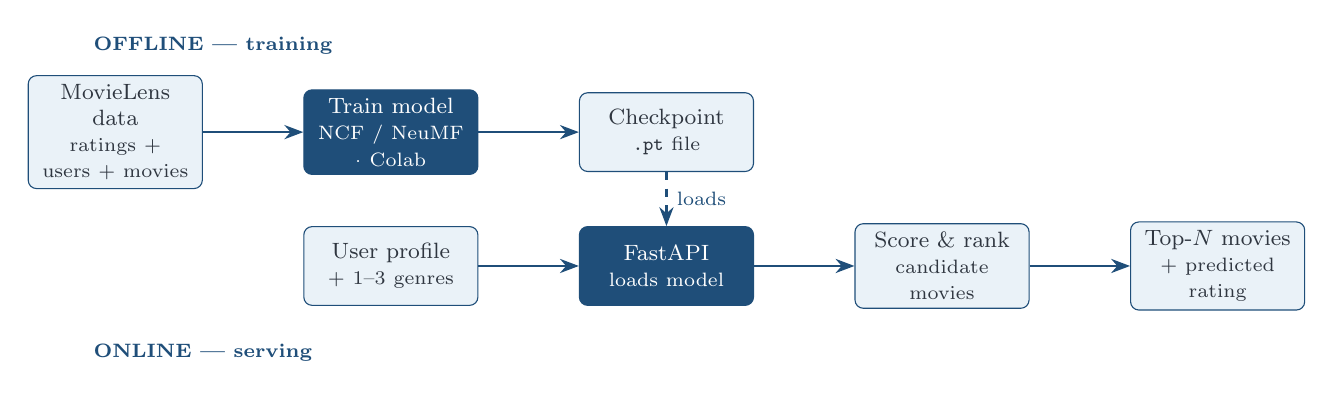
\begin{tikzpicture}[
  >=Stealth, font=\footnotesize,
  box/.style={rounded corners=3pt, draw=itcblue, fill=softblue, text=darkgray,
              minimum height=1cm, text width=2cm, align=center, inner sep=3pt},
  hi/.style={rounded corners=3pt, draw=itcblue, fill=itcblue, text=white,
             minimum height=1cm, text width=2cm, align=center, inner sep=3pt},
  arr/.style={-{Stealth[length=2.4mm]}, thick, draw=itcblue},
  phase/.style={font=\scriptsize\bfseries, text=itcblue, anchor=west}
]
% phase labels
\node[phase] at (-0.4,2.8)  {OFFLINE --- training};
\node[phase] at (-0.4,-1.1) {ONLINE --- serving};

% offline lane
\node[box] (data)  at (0,1.7)   {MovieLens data \\ {\scriptsize ratings + users + movies}};
\node[hi]  (train) at (3.5,1.7) {Train model \\ {\scriptsize NCF / NeuMF · Colab}};
\node[box] (ckpt)  at (7.0,1.7) {Checkpoint \\ {\scriptsize \texttt{.pt} file}};

% online lane
\node[box] (user)  at (3.5,0)   {User profile \\ {\scriptsize + 1--3 genres}};
\node[hi]  (api)   at (7.0,0)   {FastAPI \\ {\scriptsize loads model}};
\node[box] (rank)  at (10.5,0)  {Score \& rank \\ {\scriptsize candidate movies}};
\node[box] (top)   at (14.0,0)  {Top-$N$ movies \\ {\scriptsize + predicted rating}};

% arrows
\draw[arr] (data)  -- (train);
\draw[arr] (train) -- (ckpt);
\draw[arr, dashed] (ckpt) -- node[right, font=\scriptsize, text=itcblue] {loads} (api);
\draw[arr] (user)  -- (api);
\draw[arr] (api)   -- (rank);
\draw[arr] (rank)  -- (top);
\end{tikzpicture}%
}

\vspace{0.35cm}
{\footnotesize The checkpoint trained offline is loaded once by FastAPI, then reused to score movies for every new profile.}
\end{frame}

% ---------------------------------------------------------------------------
\begin{frame}{Challenges \& Solutions}
\centering
\renewcommand{\arraystretch}{1.5}
\small
\begin{tabular}{>{\raggedright\arraybackslash}p{4.7cm}@{\hspace{0.7cm}}>{\raggedright\arraybackslash}p{6.2cm}}
\toprule
\textbf{Challenge} & \textbf{How we solved it} \\
\midrule
Heavy PySpark \& PyTorch installs & Split \texttt{uv} dependency groups; train on Google Colab \\
Consistent encoding across the stack & One shared \texttt{features.py} reused by Spark, training \& serving \\
Messy, high-cardinality zip-codes & Collapse to the first-digit region (11 buckets) \\
Recommending to brand-new users & Demographic + genre content features instead of user IDs \\
\bottomrule
\end{tabular}
\end{frame}

% ---------------------------------------------------------------------------
\begin{frame}{Conclusion}
\begin{columns}[T]
  \begin{column}{0.32\textwidth}
    \begin{block}{Data · PySpark}
      Distributed load, join, feature engineering, split and evaluation.
    \end{block}
  \end{column}
  \begin{column}{0.32\textwidth}
    \begin{block}{Model · PyTorch}
      NCF / NeuMF learns ratings from demographics + genres, trained with DDP.
    \end{block}
  \end{column}
  \begin{column}{0.32\textwidth}
    \begin{block}{Serving · FastAPI}
      Loads the checkpoint and recommends the top-$N$ films through a web UI.
    \end{block}
  \end{column}
\end{columns}

\vspace{0.45cm}

\begin{block}{Key takeaway}
A feature-based recommender gives ranked picks to \textbf{any new viewer} from a short profile --- no rating history required --- end-to-end across PySpark, PyTorch and FastAPI.
\end{block}
\end{frame}

% ---------------------------------------------------------------------------
\begin{frame}[plain]
\begin{center}
\vspace{1.8cm}
{\Huge \bfseries Thank You}

\vspace{0.8cm}
{\Large Questions?}

\vspace{1.0cm}
{\large NGO Seakyarith \quad e20220185}\\
{\large SUM Devith \quad e20221126}\\
{\large YOS Nisiy \quad e20220287}\\
{\large RY Chhorly \quad e20220793}
\end{center}
\end{frame}

\end{document}
